\documentclass[11pt,a4paper]{article}

% --- packages ---
\usepackage[T1]{fontenc}
\usepackage[utf8]{inputenc}
\usepackage{XCharter}
\usepackage[scaled=0.86]{beramono}
\usepackage[a4paper,margin=2.3cm,top=2.1cm,bottom=2.4cm]{geometry}
\usepackage{microtype}
\usepackage{xcolor}
\usepackage{booktabs,tabularx,array}
\usepackage{enumitem}
\usepackage{titlesec}
\usepackage{amsmath}
\usepackage{tikz}
\usetikzlibrary{arrows.meta,positioning,calc}
\usepackage{fancyhdr}
\usepackage{caption}
\captionsetup{font=small,labelfont={bf,color=accent},skip=5pt,justification=raggedright,singlelinecheck=false}
\usepackage[hidelinks]{hyperref}

% --- style ---
\definecolor{ink}{HTML}{1B2430}
\definecolor{accent}{HTML}{1F4E8C}
\definecolor{muted}{HTML}{6B7480}
\definecolor{rule}{HTML}{D5DAE1}
\definecolor{soft}{HTML}{F3F5F8}

\color{ink}
\setlength{\parindent}{0pt}
\setlength{\parskip}{4pt}
\linespread{1.05}
\raggedbottom
\setlist{nosep,leftmargin=1.3em,topsep=2pt,itemsep=2pt}

\titleformat{\section}{\large\bfseries\color{accent}}{\thesection}{0.7em}{}
\titlespacing*{\section}{0pt}{13pt}{4pt}
\titleformat{\subsection}{\normalsize\bfseries}{}{0pt}{}
\titlespacing*{\subsection}{0pt}{7pt}{2pt}

\pagestyle{fancy}
\fancyhf{}
\renewcommand{\headrulewidth}{0pt}
\fancyfoot[L]{\small\color{muted}Team Ragnir \textperiodcentered{} More than a Hack 2027, Phase 1}
\fancyfoot[R]{\small\color{muted}\thepage}

\newcolumntype{L}{>{\raggedright\arraybackslash}X}
\newcommand{\lab}[1]{\texttt{#1}}
\newcommand{\note}[1]{{\small\color{muted}#1}}

\begin{document}

% --- title ---
{\color{muted}\small More than a Hack 2027 \textperiodcentered{} Phase 1: Ball Possession
\textperiodcentered{} FC Barcelona vs Athletic Club}

\vspace{4pt}
{\LARGE\bfseries Who has the ball? Possession from automatic tracking}

\vspace{6pt}
{\large Team Ragnir}

\vspace{2pt}
\note{Code: \url{https://github.com/Pers8/ragnir-possession-mtah-2027}}

\vspace{2pt}
{\color{rule}\rule{\linewidth}{0.6pt}}

% --- summary ---
\section*{Summary}

For every frame we score three options: Barcelona has the ball (\lab{H}), Athletic has it
(\lab{A}), or the ball is dead (\lab{D}). The scores come from the tracking and the Smart
Tagging. A Viterbi pass then picks the best sequence of labels for each half, with a cost for
every change of label, so possession only changes hands when the other team clearly has the
ball for long enough to pay that cost.

We went this way because the ranking metric counts whole possessions. A frame-by-frame
classifier, even a good one, flickers wherever the evidence is mixed, and every flicker splits
one possession into two. A cost on switching deals with that directly.

There is no trained model and no labels of any kind. Every constant comes from how football
works or from basic physics, and Table~\ref{tab:params} gives the reason for each one.

\begin{center}
\small
\begin{tabular}{lccc}
\toprule
Public 5-minute window & spellF1 & macroF1 & alive/dead F1 \\
\midrule
\textbf{Our submission} & \textbf{0.430} & \textbf{0.705} & \textbf{0.930} \\
Official baseline (\lab{baseline\_smooth50}) & 0.326 & 0.621 & 0.899 \\
\bottomrule
\end{tabular}
\end{center}
\note{The public window holds only 17 possessions, so these numbers show that the pipeline
works, not how it will rank. Nothing was tuned on it (Section~\ref{sec:rules}).}

% --- approach ---
\section{How it works}

\begin{center}
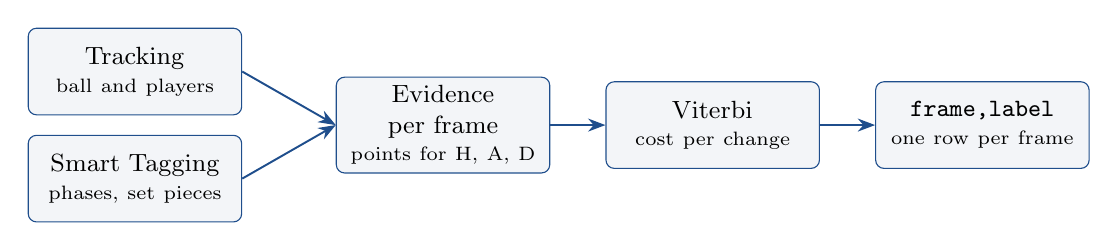
\begin{tikzpicture}[
  box/.style={draw=accent, fill=soft, rounded corners=3pt, minimum height=11mm,
              text width=25mm, align=center, font=\small, inner sep=3pt},
  arr/.style={-{Stealth[length=2.2mm]}, draw=accent, line width=0.7pt}]
  \node[box] (trk) at (0, 0.68) {Tracking\\[-1pt]{\scriptsize ball and players}};
  \node[box] (tag) at (0,-0.68) {Smart Tagging\\[-1pt]{\scriptsize phases, set pieces}};
  \node[box, anchor=west] (ev) at (2.55,0) {Evidence per frame\\[-1pt]{\scriptsize points for H, A, D}};
  \node[box, right=7mm of ev] (vit) {Viterbi\\[-1pt]{\scriptsize cost per change}};
  \node[box, right=7mm of vit] (out) {\lab{frame,label}\\[-1pt]{\scriptsize one row per frame}};
  \draw[arr] (trk.east) -- (ev.west);
  \draw[arr] (tag.east) -- (ev.west);
  \draw[arr] (ev) -- (vit);
  \draw[arr] (vit) -- (out);
\end{tikzpicture}
\end{center}

\subsection{Evidence per frame}
For each frame we add up points for \lab{H}, \lab{A} and \lab{D}. A cue adds points to the label
it supports and takes points away from the label it argues against. Most cues are worth less
than one point per frame, so a cue only matters if it holds for a while. Sections~\ref{sec:who}
and \ref{sec:dead} list every cue.

\subsection{Decoding}
\begin{minipage}[c]{0.58\linewidth}
\setlength{\parskip}{4pt}
The labels form a chain with three states. Staying in a state is free. Switching between
\lab{H} and \lab{A} costs 12 points, and going from alive to dead or back costs 20. Viterbi
finds the sequence with the highest total score, separately for each half.

Full control of the ball is worth 1 point per frame, so a turnover needs about half a second
(12 frames) of the other team clearly on the ball, and a stoppage about a second of dead-ball
cues.
\end{minipage}\hfill
\begin{minipage}[c]{0.38\linewidth}
\centering
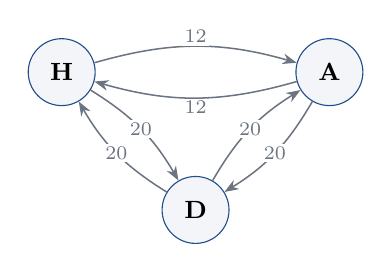
\begin{tikzpicture}[
  st/.style={circle, draw=accent, fill=soft, minimum size=8.5mm, font=\small\bfseries},
  e/.style={-{Stealth[length=1.8mm]}, draw=muted, line width=0.55pt},
  lbl/.style={font=\scriptsize, color=muted, fill=white, inner sep=1pt}]
  \node[st] (H) at (0,0) {H};
  \node[st] (A) at (3.4,0) {A};
  \node[st] (D) at (1.7,-1.75) {D};
  \draw[e, bend left=16] (H) to node[lbl, above] {12} (A);
  \draw[e, bend left=16] (A) to node[lbl, below] {12} (H);
  \draw[e, bend left=14] (H) to node[lbl] {20} (D);
  \draw[e, bend left=14] (D) to node[lbl] {20} (H);
  \draw[e, bend left=14] (A) to node[lbl] {20} (D);
  \draw[e, bend left=14] (D) to node[lbl] {20} (A);
\end{tikzpicture}

\note{\scriptsize Cost of each change of label}
\end{minipage}

% --- data ---
\section{Data we used}

\begin{center}
\small
\begin{tabularx}{\linewidth}{@{}p{4.1cm}L@{}}
\toprule
Asset & How we used it \\
\midrule
Tactical tracking & Ball position, distance from the ball to each team, player speeds, team shape \\
Tracking metadata & Which track slot belongs to which team \\
Smart Tagging & Which team is attacking, and where set pieces start \\
Homography & Not needed: the tracking is already in pitch coordinates \\
Video, broadcast tracking & Not used. The broadcast feed is not synchronised, and we had no
external data to build a video model with \\
\bottomrule
\end{tabularx}
\end{center}

% --- who has the ball ---
\section{Who has the ball}\label{sec:who}

\begin{itemize}
  \item \textbf{Control.} A player within 2\,m of the ball who is clearly closer than any
  opponent gives their team 1 point.
  \item \textbf{Duels.} If players from both teams are within 1\,m of each other near the
  ball, nobody gets the point. A challenge on its own does not change possession.
  \item \textbf{Closer team.} Otherwise the closer team gets a small bonus, up to 0.2 points,
  growing with the gap in distance up to 5\,m. Beyond that, being closer says very little,
  for example while a long pass is in the air.
  \item \textbf{Smart Tagging.} An attacking phase gives its team 0.15 points, and a defending
  phase gives the same to the other team. The tags are automatic and cover 5 to 35 seconds at
  a time, so they only tip close calls.
  \item \textbf{Team shape, only when the ball is not seen.} A team with the ball spreads out
  to make space and a team without it closes up. We measure each team's spread as the mean
  distance of its players to their centre, leaving out the player furthest away (usually the
  goalkeeper). A 2.5\,m difference in spread counts as one unit, capped at two, and the cue
  moves at most 0.15 points either way. It is only used when the ball is unseen or out of play,
  and it only moves points between \lab{H} and \lab{A}, never towards or away from \lab{D}.
\end{itemize}

To check that team shape is a real signal, we took the frames where the tracking itself shows
one player clearly on the ball. On those frames the wider team was the team in control 76\% of
the time. This was a check only; nothing was fitted to it.

% --- dead ball ---
\section{Is the ball dead}\label{sec:dead}

\subsection{General cues}
\begin{itemize}
  \item The ball is seen outside the lines: strong dead-ball evidence.
  \item The ball has not been seen for most of a 2-second stretch: some dead-ball evidence.
  \item Player speed, averaged over one second. Normal walking pace is about 1.4\,m/s. Below
  1.0\,m/s the players are standing or strolling, which happens at stoppages. Above 1.6\,m/s
  they are moving faster than a walk, so play is live.
\end{itemize}

\subsection{Restarts}
The Smart Tagging marks 59 set pieces, but a match has well over a hundred restarts (around 40
throw-ins alone). So we also look for restarts in the tracking:

\begin{itemize}
  \item \textbf{Ball going out.} The ball is last seen within 3\,m of a line, moving towards
  it at 2\,m/s or more, and then disappears. The whole gap counts as dead.
  \item \textbf{Ball placed.} The ball is visible but slower than 1\,m/s for about a second,
  as before a free kick, a goal kick or a corner.
  \item \textbf{Taker outside the line.} A player stands at least 0.5\,m beyond a line within
  2\,m of the ball, as for a throw-in or a corner.
  \item \textbf{Tagged set pieces.} From the start of the tag, the ball is dead until it is
  struck: half a second of the ball resting (unseen or slower than walking pace), then faster
  than 5\,m/s for two frames, looking at most 15\,s ahead. This finds the kick in 41 of the
  59 tagged set pieces. When no kick is found, the tag adds no dead time.
  \item \textbf{Goals.} The 30 seconds before a kick-off after a goal are dead (celebration
  and checks).
\end{itemize}

% --- rules of possession ---
\section{Possession rules}

\begin{itemize}
  \item \textbf{Loose balls and passes.} If nobody is near the ball there is no new evidence,
  so the team that last had it keeps possession until the other side clearly controls it.
  \item \textbf{Challenges.} A duel gives no evidence, so possession only changes once someone
  comes out of it with the ball.
  \item \textbf{Turnovers.} The other team has to clearly control the ball for about half a
  second before we switch.
  \item \textbf{Restarts.} The ball is dead from the moment it leaves the pitch, or play stops,
  until the restart is taken. Who takes the restart does not matter: it is \lab{D}.
  \item \textbf{Outside the halves.} Before kick-off, at half-time and after the final
  whistle we write \lab{X}.
\end{itemize}

% --- parameters ---
\begin{table}[t]
\caption{Every parameter and why we picked its value. All of them live in \lab{PARAMS} at the
top of \lab{solution/run.py}.}\label{tab:params}
\small
\begin{tabularx}{\linewidth}{@{}p{3.2cm}p{3.0cm}L@{}}
\toprule
Parameter & Value & Why \\
\midrule
Control radius & 2\,m & A player can reach a ball about a stride away \\
Duel gap & 1\,m & Both teams that close means the ball is contested \\
Distance cap & 5\,m & Further than that, being closer says little \\
Switch cost & 12 & About half a second of clean control before a turnover \\
Alive/dead cost & 20 & Stoppages last seconds, not single frames \\
Slow / fast players & 1.0 / 1.6\,m/s & Either side of normal walking pace (1.4\,m/s) \\
Ball placed & $<$1\,m/s for 1\,s & A rolling or passed ball is faster than walking pace \\
Kick & $>$5\,m/s & Even a soft pass or a throw-in travels faster than this \\
Ball going out & $\le$3\,m, $\ge$2\,m/s & A ball heading out that is then lost has almost always crossed the line \\
Taker outside & 0.5\,m out, ball $\le$2\,m & A throw-in taker stands behind the line holding the ball \\
Goal celebration & 30\,s & Restarts after a goal never come sooner \\
Team shape unit & 2.5\,m, cap 2 & A few metres of difference in spread is already clear \\
Tag weights & 0.15 to 0.6 & Weaker than tracking: the tags are automatic and coarse \\
\bottomrule
\end{tabularx}
\end{table}

% --- results ---
\section{Results}

\begin{center}
\small
\begin{tabularx}{\linewidth}{@{}p{1.1cm}Lccc@{}}
\toprule
Version & What changed & spellF1 & macroF1 & alive/dead F1 \\
\midrule
v1 & Distances, ball out, player speed, tags, Viterbi & 0.385 & 0.596 & 0.907 \\
v2 & Restart detection from the tracking, goal rule & 0.430 & 0.704 & 0.930 \\
Final & Team shape, kick detection, no fitted parts & \textbf{0.430} & \textbf{0.705} & \textbf{0.930} \\
\midrule
 & Official baseline (\lab{baseline\_smooth50}) & 0.326 & 0.621 & 0.899 \\
\bottomrule
\end{tabularx}
\end{center}
\note{Scores on the public 5-minute window. Over the full match, where there is no ground
truth, we find 241 possessions and 109 stoppages, both in the range a real match has.}

% --- rules ---
\section{Staying within the rules}\label{sec:rules}

We followed the organisers' clarification of 3 November.

\begin{itemize}
  \item \textbf{No labels, no training, no tuning.} Nothing in the pipeline is fitted to this
  match, to the ground truth or to the video. Every constant was chosen from football
  knowledge or physics.
  \item \textbf{The public ground truth was only a check.} We scored each version on the
  public window once it was finished, to make sure nothing was broken. We never searched
  values against it.
  \item \textbf{Automatic checks on the provided data only.} The team-shape check (76\%) and
  the kick count (41 of 59) use the tracking and the tags, never the ground truth.
  \item \textbf{What we changed to follow the clarification.} An earlier version fitted a
  small logistic regression for team shape on this match's tracking, and set the set-piece
  delay from the two tagged kick-offs. We replaced both with the fixed rules above, and the
  public-window scores did not change. The walking-pace thresholds were first read off this
  match's speed distribution; they are now based on normal walking pace and kept the same
  values. An early draft used a switch cost of 25 (a full second of control); we lowered it to
  12 because it gave possessions longer than typical football, judged on our own output only.
  \item \textbf{AI assistance.} We used an AI assistant (Claude) to help write code and this
  report. None of the match data was uploaded to it: it only saw summary numbers printed by
  our scripts, such as counts, percentiles and scores.
\end{itemize}

% --- limitations ---
\section{Limitations and next steps}

\begin{itemize}
  \item \textbf{Fouls and offsides.} Play stops while the ball is still inside the pitch and
  often still moving, so we only notice once the ball is placed. The referee's whistle in the
  video audio would give the exact moment.
  \item \textbf{Quick turnovers.} A one-touch interception rarely shows half a second of clean
  control, so some short possessions merge into their neighbours.
  \item \textbf{Hidden ball at a turnover.} When the ball is not seen as it changes hands, the
  switch can land a little late.
  \item \textbf{Hand-set weights.} With labelled data from other matches, the weights and costs
  could be learned instead of set by hand.
\end{itemize}

% --- reproduction ---
\section{Reproduction}

\colorbox{soft}{\parbox{\dimexpr\linewidth-2\fboxsep}{\small\ttfamily
pip install -r requirements.txt\\
python solution/run.py -{}-team Ragnir\\
python -m unittest discover tests}}

\vspace{2pt}
The second command writes the submission and runs the official validator, and the third runs
our unit tests. Input goes in \lab{data/tactical/} and the output in
\lab{evaluation/results/}. There is no randomness, so the same data always gives the same
file. Tested with Python 3.11, numpy 2.4.6 and pandas 3.1.1.

\end{document}
